\chapter{定式化}\label{formulation}

この章では1節で本研究における記号の定義や問題の定式化について説明し, 2節では, 本研究に関連する詰込み問題の説明をする. 
その後に, 本問題に関する独自の制約や目的関数を説明し, 定式化する. \\

\section{記号の定義}

\begin{table}[htb]
    \begin{center}
    \label{table31}
    \begin{tabular}{cp{35em}} \hline
    記号 & \hspace{2.0em}記号の説明 \\ \hline

    $x_i$ &
    \begin{tabular}{l}
    \hspace{1.4em}長方形$i$の左下のx座標
    \end{tabular} \\ \hline

    $y_i$ &
    \begin{tabular}{l}
    \hspace{1.4em}長方形$i$の左下のy座標
    \end{tabular} \\ \hline    
    
    $w_i$ &
    \begin{tabular}{l}
    \hspace{1.4em}長方形$i$の幅
    \end{tabular} \\ \hline

    $w_i^l$ &
    \begin{tabular}{l}
    \hspace{1.4em}長方形$i$の幅の下界
    \end{tabular} \\ \hline

    $w_i^u$ &
    \begin{tabular}{l}
    \hspace{1.4em}長方形$i$の幅の上界
    \end{tabular} \\ \hline

    $h_i$ &
    \begin{tabular}{l}
    \hspace{1.4em}長方形$i$の高さ
    \end{tabular} \\ \hline

    $h_i^l$ &
    \begin{tabular}{l}
    \hspace{1.4em}長方形$i$の高さの下界
    \end{tabular} \\ \hline

    $h_i^u$ &
    \begin{tabular}{l}
    \hspace{1.4em}長方形$i$の高さの上界
    \end{tabular} \\ \hline
    
    $W$ &
    \begin{tabular}{l}
    \hspace{1.4em}母材の横幅
    \end{tabular} \\ \hline
    $H$ &
    \begin{tabular}{l}
    \hspace{1.4em}母材の高さ
    \end{tabular} \\ \hline
    $S_i$ &
    \begin{tabular}{l}
    \hspace{1.4em}長方形$i$の面積
    \end{tabular} \\ \hline
    $I$ &
    \begin{tabular}{l}
    \hspace{1.4em}詰め込む長方形の集合
    \end{tabular} \\ \hline
    $\overline{I}$ &
    \begin{tabular}{l}
    \hspace{1.4em}既配置の長方形の集合\ $\overline{I} \subseteq I$
    \end{tabular} \\ \hline
    $J$ &
    \begin{tabular}{l}
    \hspace{1.4em}障害物の集合
    \end{tabular} \\ \hline
    
    
    \end{tabular}
    \end{center}
    \end{table}

\section{一般論(仮タイトル)}

\subsection{長方形詰込み問題}
長方形詰込み問題とは, 母材の幅$W$と高さ$H$, 長方形集合$I$に対し, 幅$w_i$, 高さ$h_i$が入力として与えられ, 母材からはみ出ることなくまた, どの二つの長方形も互いに重なることがないように詰め込む問題である. \\
以上の条件を定式化すると, 次のように書くことができる. \\
\textgt{条件1: 長方形$i \in I$は母材上に配置される. }\\
\begin{eqnarray}
    0 \leq x_i \leq W-w_i \ (i \in I), \\
    0 \leq y_i \leq H-h_i \ (i \in I). 
\end{eqnarray}
\textgt{条件2: 長方形$i,j \in I$は互いに重ならない. }\\
この条件は, 次の4つの不等式のうち一つ以上が成立しなければいけない.  
\begin{eqnarray}
    x_i + w_i \leq x_j \ (i \in I), \\
    x_j + w_j \leq x_i \ (i \in I), \\
    y_i + h_i \leq y_j \ (i \in I), \\
    y_j + h_j \leq y_i \ (i \in I). 
\end{eqnarray}

\subsection{Soft-rectangleパッキング問題}
長方形詰込み問題の一種で, 詰め込む長方形の幅と高さを可変としたsoft-rectangle (可変形状長方形)を扱う\cite{soft-rectangle}. 
長方形$i \in I$の座標$x_i,y_i$だけでなく幅$w_i$と高さ$h_i$も変数とする. \\
通常, 長方形$i \in I$の面積に関する次のような等式制約または不等式制約が存在する: \\
\begin{eqnarray}
    w_i * h_i = S_i, \\
    w_i * h_i \geq S_i. \\
\end{eqnarray}
また, 長方形 $i \in I$の幅と高さの上界, 下界に関する以下の制約も存在する: 
\begin{eqnarray}
    w_i^l \leq w_i \leq w_i^u, \\
    h_i^l \leq h_i \leq h_i^u. 
\end{eqnarray}

\subsection{Sequence-pair}
Sequence-pairとは, 二つの順列による長方形の配置表現である\cite{seq-pair}. 
長方形同士の相対位置関係を長方形名の順列対により表すことができる. 
例を図\ref{s-p-eg}に示す. 制約の詳細は3.3節で説明する. 
Sequence-pairはどのような配置表現でも一意の順列対に表現でき, 逆に任意の順列対から一意に配置表現を求めることができる. \\ 

\begin{figure}[b]
    \hspace{2cm}
    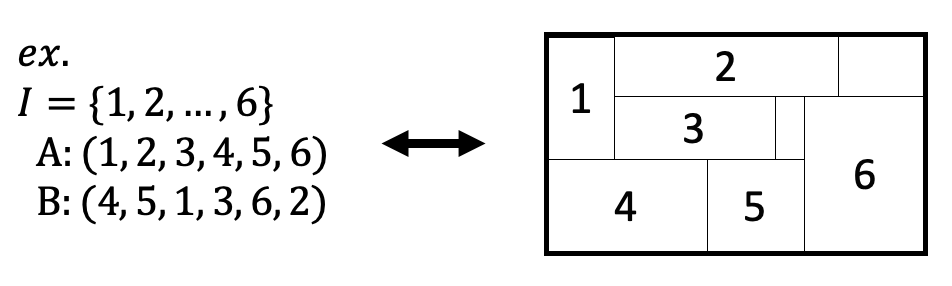
\includegraphics[scale=0.3, bb = 0 0 1 1]{3-sequence-pair.png}
    \caption{sequence-pairによる長方形配置表現}
    \label{s-p-eg}
\end{figure}
\clearpage

\subsection{No-fit polygon}
No-fit polygon (NFP)とは, 平面上で多角形の重なりを判定する方法である\cite{nfp}\cite{nfp2}. 
多角形$P$と$Q$が与えられ, $Q$の配置が固定されているとする. 
この時, 多角形$P$が$Q$と重なりを持つ領域をNFP($P,Q$)と書き, 図\ref{nfp-eg}に示す. 
図\ref{nfp-eg}の太線がNFPの境界を表し, このNFP内に$P$を配置すると$Q$と重なることを意味する. 
母材内の既配置の長方形全てに対し, 長方形$i$のNFPを作成すると, 長方形$i$の配置可能領域はどのNFPの内部にも含まれない領域である. \\


\begin{figure}[tbp]
    \hspace{3cm}
    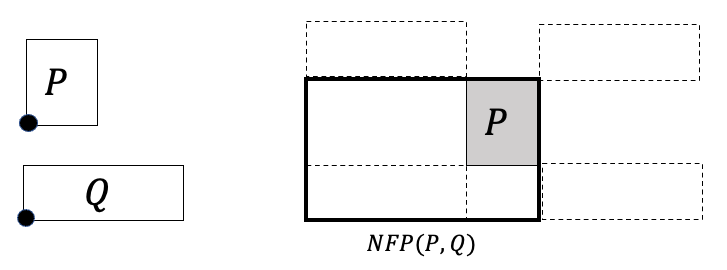
\includegraphics[scale = 0.3, bb=0 0 10 10]{3nfp.png}
    \caption{NFP($P,Q$)}
    \label{nfp-eg}
\end{figure}

\section{第一段階}
第一段階では, 積み地・揚げ地が同じ車を一つのグループとし, 各グループのデッキ内における大まかな配置場所を決定する. 
グループ内の車の総面積を計算し, soft-rectangleパッキング問題として定式化する. 
このパッキングはセグメントごとに行う. 

\subsection{制約}
\textgt{(i)ランプから配置場所までの移動経路確保に関する制約}\\
\ プランナーへのヒアリングの結果から, 先に積む貨物ほど入口から見て奥に積み, 後から積む貨物ほど手前に積むことが望ましいと分かった. 
同様に, 先に降ろす貨物ほど入口から見て手前に積み, 後から下ろす荷物ほど奥に積むこともまた望まれる. 
本研究では, Sequence-pairを用いてグループの相対位置関係に関する制約を表現する. 
各グループを積み地の昇順に並べた順列を$\sigma^+$とする. 
積み地が同じグループが存在した場合, 揚げ地の降順に従う. 
同様に, 揚げ地の降順に並べた順列を$\sigma^-$とする. 
揚げ地が同じグループが存在する場合, 積み地の昇順に従う. \\
グループの集合を$I$とし, グループ$i,j \in I$に関して, 順序対$(\sigma^+,\sigma^-)$における$i,j$の順序関係をもとに, 以下のどちらかの制約を追加する: \\
\begin{eqnarray}
    \left\{
        \begin{array}{ll}
            y_i + h_i \leq y_j & \sigma^+(\ldots,i,\ldots,j,\ldots) \cap \sigma^-(\ldots,i,\ldots,j,\ldots) \\
            x_i + w_i \leq x_j & \sigma^+(\ldots,i,\ldots,j,\ldots) \cap \sigma^-(\ldots,j,\ldots,i,\ldots) \\
        \end{array}
    \right.
\end{eqnarray}\\


\textgt{(ii)各グループの面積に関する制約}\\
\ 次の段階で各グループの車を詰め込むためには, グループの面積はグループ内に属する車の総面積よりも大きくなければいけない. 
以上の制約は, グループの集合を$I$とし, グループ$i \in I$の車の総面積を$S_i$とすると, 以下のように書ける: \\
\begin{eqnarray}
    w_i*h_i \geq S_i , 
\end{eqnarray}
一つのグループの領域が大きくなりすぎると, デッドスペースが生まれたり, 他のグループの領域で詰め込めない車が出てしまう可能性があるので, パラメータ変数$a\ (a \geq 1)$を用意して, 以下のように上から抑える. 
\begin{eqnarray}
    w_i*h_i \leq a*S_i.
    \label{a_const}
\end{eqnarray}\\

\textgt{(iii)各グループの幅と高さに関する制約}\\
\ 各グループ$I$の幅と高さは, グループ内に属する車$i \in I$の幅と長さの最大値をもとに以下の下限を設定する: \\
\begin{eqnarray}
    w_I \geq \max_{i \in I} w_i, \\
    h_I \geq \max_{i \in I} h_i. 
\end{eqnarray}


\subsection{目的関数}
目的関数として, デッキ内のより多くの領域を配置可能場所として使えることが望ましいので, グループの面積和の最大化を目指す. 
また1つのグループが大きくなりすぎると, デッドスペースが生まれたり, 他のグループの領域で詰め込めない車が出てしまう可能性があるので, バランス良く大きくすることを目指す. 
面積制約\ref{a_const}で用いたパラメータ$a$を用いて, 以下のように書くことができる: \\
\begin{eqnarray}
    \mathrm{maximize}\ \sum_{i \in I} w_i*h_i  - a. 
\end{eqnarray}
\subsection{定式化}
パッキングするグループの集合を$I$とし, セグメントの幅と高さをそれぞれ$W, H$とし, 以上をまとめると以下のようになる. \\
\begin{center}
    \begin{align}
        & \textrm{maximize} \hspace{1.5cm}
        \sum_{i \in I} w_i - h_i - a \\
        & \textrm{subject\ to} \hspace{1.5cm}
        0 \leq x_i \leq W - w_i & (i \in I) \\
        &\hspace{3cm} 0 \leq y_i \leq H - y_i & (i \in I) \\
        &\hspace{3cm} 0 \leq w_i \leq \max_{car \in i}w_{car} & (i \in I) \\
        &\hspace{3cm} 0 \leq h_i \leq \max_{car \in i}h_{car} & (i \in I) \\
        &\hspace{2.8cm} S_i \leq w_i*h_i \leq a*S_i &(i \in I)
    \end{align}
    \begin{eqnarray}
        \hspace{2cm} \left\{
            \begin{array}{ll}
                y_i + h_i \leq y_j & \sigma^+(\ldots,i,\ldots,j,\ldots) \cap \sigma^-(\ldots,i,\ldots,j,\ldots) \\
                x_i + w_i \leq x_j & \sigma^+(\ldots,i,\ldots,j,\ldots) \cap \sigma^-(\ldots,j,\ldots,i,\ldots) \\
            \end{array}
        \hspace{2cm} \right.
    \end{eqnarray}
\end{center}

\section{第二段階}
第二段階では, 第一段階で決められた領域をはみ出ることがないように, 車一台ずつの配置場所を決定する. 
車を長方形に近似することで, 長方形詰込み問題として定式化する. 

\subsection{制約}
\textgt{(i)駐車に必要な局所的なスペースに関する制約}\\
\ 駐車は原則バック駐車で行うため, 配置位置周辺に局所的なスペースが必要となる. 
例えば, 配置位置のすぐ前方に柱等の障害物があると, 配置図上では配置可能に見えても, 実際には障害物が邪魔で駐車できない可能性がある.
この点を考慮するため, 予め駐車に必要なスペースを定義する.
プランナーへのヒアリングの結果から, 駐車にはおおよそ車体長さの半分に相当するスペースが必要で, このスペース上に障害物がなければ良いということが分かった. 
車$i$の大きさと駐車に必要なスペースを合わせたレクトリニア図形を$f(i)$で定義する. 
障害物の集合を$J$, 既配置の車の集合を$\overline{I}$とすると, 車$i$の配置不可能な領域はNFPの表現を用いて以下のように書くことができる.  
\begin{eqnarray}
    \label{nfp-eq1}
    \sum_{j \in J} NFP(f(i),j) + \sum_{\overline{i} \in \overline{I}} NFP(f(i),\overline{i})
\end{eqnarray}\\

\textgt{(ii)配置間隔に関する制約}\\
配置される車の間隔は他の車両や障害物と前後方向に30 cm, 左右方向に10 cm空いている必要がある. 
また, オペレーターの乗り降りのため, 左右の内ハンドル側に40 cm空いている必要がある. 
先ほどの制約同様, 配置予定の車を上記の単位だけ大きくしてNFPを計算する. 
車両$i$を上下方向に30 cmずつ, 左右方向に10 cmずつ, ハンドル側を40 cm大きくした長方形を$g(i)$とすると, 車両$i$の配置不可能な領域は以下のように表される. 
\begin{eqnarray}
    \label{nfp-eq2}
    \sum_{j \in J} NFP(g(i),j) + \sum_{\overline{i} \in \overline{I}} NFP(g(i),\overline{i})
\end{eqnarray}

車両$i$が配置可能な領域は, (\ref{nfp-eq1}), (\ref{nfp-eq2})以外の領域である. 

\subsection{目的関数}
第二段階では, 目的関数の設定は行わず解の構築のみを行う. 

\subsection{定式化}
まとめると, グループ$I$内の車$i$をパッキングする時の制約は, 以下のようになる. 
\begin{center}  
\begin{align}
    & \textrm{subject\ to} \hspace{1cm}0 \leq x_i \leq W_I - w_i & (i \in I)\\
    & \hspace{2.6cm} 0 \leq y_i \leq H_I - h_i & (i \in I)\\
    & \hspace{2.6cm} x_i + w_i \leq x_j \hspace{0.3cm}or\hspace{0.3cm} x_j + w_j \leq x_i \hspace{0.3cm}or \nonumber \\
    & \hspace{2.6cm} y_i + h_i \leq y_j \hspace{0.3cm}or\hspace{0.3cm} y_j + h_j \leq y_i &(i,j \in I)\\
    & \hspace{2cm} (x_i, y_i) \neq \sum_{j \in J} NFP(f(i)+g(i),j) + \sum_{\overline{i} \in \overline{I}}NFP(f(i)+g(i),\overline{i}) & (i \in I)
\end{align}
\end{center}